\fenicschapter{Turbulent Flow and Fluid-Structure Interaction with Unicorn}
              {Turbulent Flow and Fluid-Structure Interaction with Unicorn}
              {Johan Hoffman, Johan Jansson, Niclas Jansson, Claes Johnson and Murtazo Nazarov}
              {hoffman-1}

\section{Introduction}

For many problems involving a fluid and a structure, decoupling the
computation of the two is not possible for accurate modeling of the
phenomenon at hand, instead the full fluid-structure interaction (FSI)
problem has to be solved together as a coupled problem. This includes
a multitude of important problems in biology, medicine and industry,
such as the simulation of insect or bird flight, the human
cardiovascular and respiratory systems, the human speech organ, the
paper making process, acoustic noise generation in exhaust systems,
airplane wing flutter, wind induced vibrations in bridges and wave
loads on offshore structures. Common for many of these problems is
that for various reasons they are very hard or impossible to
investigate experimentally, and thus reliable computational simulation
would open up for detailed study and new insights, as well as for new
important design tools for construction.

Computational methods for FSI used today are characterized by a high
computational cost, and a lack of generality and reliability. In
particular, major open challenges of computational FSI include: (i)
robustness of the fluid- structure coupling, (ii) for high Reynolds
numbers the computation of turbulent fluid flow, and (iii) efficiency
and reliability of the computations in the form of adaptive methods
and quantitative error estimation.

The FEniCS project aims towards the goals of generality, efficiency,
and simplicity, concerning mathematical methodology, implementation,
and application.  The Unicorn project is a realization of this effort
in the field of continuum mechanics, with a range of challenging
problems that traditionally demand a number of specialized methods and
codes.  The basis of Unicorn is an adaptive finite element method and
a unified continuum formulation, which offer new possibilities for
computational modeling of high Reynolds number turbulent flow, gas
dynamics and fluid-structure interaction.

Unicorn, which is based on the DOLFIN/FFC/FIAT suite, and PETSc for
linear algebra, is today central in a number of applied research
projects, characterized by large problems, complex geometry and
constitutive models, and a need for results with quantitative error
control.  We here present some key elements of Unicorn and the
underlying theory, and illustrate how this opens for a number of
breakthroughs in applied research. The Unicorn implementation is
described in detail in Chapter~\ref{chapter:implementation:unicorn}.

\section{Continuum mechanics models}

Continuum mechanics is based on conservation laws for mass, momentum
and energy, together with constitutive laws for stresses. A Newtonian
fluid is characterized by a linear relation between the viscous stress
and the strain, together with a fluid pressure, resulting in the
Navier-Stokes equations.  Many common fluids, including water and air
at subsonic velocities, can be modeled as incompressible fluids, where
the pressure acts as a Langrangian multiplier enforcing a divergence
free velocity. In models of gas dynamics the pressure is given from
the internal energy, with an ideal gas corresponding to a linear
relation.  Solids and non-Newtonian fluids can be described by
arbitrary complex laws relating the stress to displacements, strains
and internal energies.

Newtonian fluids are characterized by two important non-dimensional
numbers: the Reynolds number $Re$, measuring the importance of viscous
effects, and the Mach number $M$, measuring compressibility effects by
relating the fluid velocity to the speed of sound. High $Re$ flow is
characterized by partly turbulent flow, and high $M$ flow by shocks
and contact discontinuities, all phenomena associated with complex
flow on a range of scales. The Euler equations corresponds to the
limit of inviscid flow where $Re \rightarrow \infty$, and
incompressible flow corresponds to the limit of $M\rightarrow 0$.

In this Chapter we focus on incompressible fluids, and leave a
discussion on compressible fluids to
Chapter~\ref{chapter:applications:thermo}

\section{Mathematics framework for fluid mechanics}

The mathematical theory for the Navier-Stokes equations is incomplete,
without any proof of existence or uniqueness, formulated as one of the
Clay Institute \$1 million problems.  What is available, is the proof
of existence of weak solutions by Leray from 1934, but this proof does
not extend to the inviscid case of the Euler equations.  No general
uniqueness result is available for weak solutions, which limit the
usefulness of the concept.

In \cite{HoffmanJohnson2008}, weak (output) uniqueness is introduced,
to characterize well-posedness of weak solutions with respect to
functionals $M(u)$ of the solution $u$. This framework extends to the
Euler equations, and also to compressible flow. The basic result takes
the form
\begin{equation}
\vert M(u) - M(U) \vert \leq S (\Vert R(u)\Vert_{-1} + \Vert R(U)\Vert_{-1})
\end{equation}
with $\Vert \cdot \Vert _{-1}$ a weak norm measuring residuals $R(\cdot)$ of two weak solutions $u$ and
$U$, and with $S$ a stability factor given by a duality argument connecting local errors to output errors
in $M(\cdot)$.

\section{Adaptive computational fluid modeling}

Computational methods in fluid mechanics are typically very
specialized; for a certain range of $Re$ or $M$, or for a particular
class of geometries. In particular, there is a wide range of
turbulence models and shock capturing techniques.

The goal of Unicorn is to design one method with one implementation,
capable of modeling general geometry and the whole range of parameters
$Re$ and $M$. We use the mathematical framework of well-posedness as a
general foundation for Newtonian fluid mechanics, where a General
Galerkin (G2) finite element method offers a robust algorithm to
compute weak solutions \cite{HoffmanJohnson2006}.  The UFL
implementation of a G2 method in Unicorn is shown in
Fig.\ref{code:ICNS}.

Adaptive G2 methods developed
in \cite{HoffmanJohnson2006a,Hoffman2005,Hoffman2009,Hoffman2006} are
based on a posteriori error estimates of the form:
\begin{equation}
\vert M(u) - M(U) \vert \leq \sum_K {\cal E}_K
\end{equation}
with $M(u)$ the target output to compute and $M(U)$ the approximation,
with $u$ and $U$ G2 solutions, and ${\cal E}_K$ a local error
indicator for cell $K$.  The error indicator ${\cal E}_K$ is
constructed as from the residual, measuring local errors, weighted by
the solution to a dual (adjoint) problem measuring the effect of local
errors on the output $M(\cdot)$. The UFL implementation of the dual
problem in Unicorn is shown in Fig.\ref{code:DUALICNS}

The computational mesh is then modified according to $ {\cal E}_K$, by
mesh refinement, coarsening or smoothing. The algorithms underlying
the parallel implementation the adaptive algorithm is described in
detail in Chapter~\ref{chapter:algorithms:parallel}.

\section{Turbulent boundary layers}
\label{section:blayer}

The choice of boundary conditions at a solid wall is critical for
accurate modeling of fluid flow, in particular to capture flow
separation phenomena. Since full resolution of a turbulent boundary
layers is out of reach, the standard way to handle the problem is to
divide the computational domain into: (i) an interior part $\Omega$,
and (ii) a boundary layer.  In the boundary layer a simplified model
of the flow is used to provide boundary conditions to the
Navier-Stokes equations to be solved in the interior part
$\Omega$. Boundary conditions may be in the form of velocities or
stresses, and the coupling between (i) and (ii) may be one-way from
(ii) to (i), or more closely coupled. Boundary layer models are
developed based on experimental data, theory or computation (in a
multiscale framework). For an overview of boundary layer modeling, see
e.g. \cite{Sagaut2005,SagautDeckTerracol2006}.

Turbulent boundary layer modeling in Unicorn is based on recent
work \cite{Hoffman2009,Hoffman2006c,HoffmanJohnson2008b,JanssonHoffman2009}
where the turbulent boundary layer is modelled by a skin friction
stress at the boundary. That is, we append the Navier-Stokes equations
with the following boundary conditions for the velocity $u$ and stress
$\sigma$:
\begin{eqnarray}
&&u\cdot n=0, \label{slfra} \\ &&u\cdot \tau _k + \beta
^{-1}n^T\sigma \tau _k=0,\quad k=1,2, \label{slfrb}
\end{eqnarray}
for $(x,t)\in \Gamma_{solid}\times [0,T]$, with $n=n(x)$ an outward
unit normal vector, and $\tau_k=\tau_k(x)$ orthogonal unit tangent
vectors of $\Gamma_{solid}$. We use matrix notation with all vectors
$v$ being column vectors and the corresponding row vector is denoted
$v^T$. For a tangent velocity $u\cdot \tau_k \sim 1$, the friction
parameter $\beta \sim F_f$, with $F_f$ the skin friction stress. The
weak implementation of the skin friction boundary condition in Unicorn
is shown in Fig.\ref{code:ICNS}.

\begin{figure}[h]
  \begin{python}
scalar = FiniteElement("Lagrange", tetrahedron, 1)
vector = VectorElement("Lagrange", tetrahedron, 1)
constant_scalar = FiniteElement("Discontinuous Lagrange", tetrahedron, 0)
constant_vector = VectorElement("Discontinuous Lagrange", tetrahedron, 0)

v      = TestFunction(vector)      # test basis function
U      = TrialFunction(vector)     # trial basis function
um     = Function(vector)          # cell mean linearized velocity
u0     = Function(vector)          # velocity from previous time step
f      = Function(vector)          # force term
p      = Function(scalar)          # pressure
delta1 = Function(constant_scalar) # stabilization parameter
delta2 = Function(constant_scalar) # stabilization parameter
tau_1  = Function(vector)          # force term
tau_2  = Function(vector)          # force term
beta  = Function(scalar)           # friction parameter

k  = Constant(tetrahedron) # time step
nu = Constant(tetrahedron) # viscosity

i0 = Index()    # index for tensor notation
i1 = Index()    # index for tensor notation
i2 = Index()    # index for tensor notation

# Galerkin discretization of bilinear form
G_a  = (inner(v, U) + k*nu*0.5*inner(grad(v), grad(U)) \
   	+ 0.5*k*v[i0]*um[i1]*U[i0].dx(i1))*dx \
  	 + 0.5*k*beta*(inner(U,tau_1)*inner(v,tau_1) \
  	 + inner(U,tau_2)*inner(v,tau_2))*ds

# Least squares stabilization of bilinear form
SD_a = (delta1*k*0.5*um[i1]*v[i0].dx(i1)*um[i2]*U[i0].dx(i2) \
           + delta2*k*0.5*div(v)*div(U))*dx

# Galerkin discretization of linear form
G_L  = (inner(v, u0) + k*inner(v, f) + k*div(v)*p \
          - k*nu*0.5*inner(grad(v), grad(u0)) \
          - 0.5*k*v[i0]*um[i1]*u0[i0].dx(i1))*dx \
          - 0.5*k*beta*(inner(u0,tau_1)*inner(v,tau_1) \
          + inner(u0,tau_2)*inner(v,tau_2))*ds

# Least squares stabilization of linear form
SD_L = (- delta1*k*0.5*um[i1]*v[i0].dx(i1)*um[i2]*u0[i0].dx(i2) \
           - delta2*k*0.5*div(v)*div(u0))*dx

# Bilinear and linear forms
a = G_a + SD_a
L = G_L + SD_L
\end{python}
\caption{Source code for bilinear and linear forms for solving the incompressible Navier-Stokes equations.}
\label{code:ICNS}
\end{figure}

\begin{figure}[!h]
\begin{python}
scalar = FiniteElement("Lagrange", tetrahedron, 1)
vector = VectorElement("Lagrange", tetrahedron, 1)
constant_scalar = FiniteElement("Discontinuous Lagrange", tetrahedron, 0)
constant_vector = VectorElement("Discontinuous Lagrange", tetrahedron, 0)

v      = TestFunction(vector)      # test basis function
U      = TrialFunction(vector)     # trial basis function
um     = Function(vector)          # primal velocity
u0     = Function(vector)          # velocity from previous time step
f      = Function(vector)          # force term
p      = Function(scalar)          # pressure
delta1 = Function(constant_scalar) # stabilization parameter
delta2 = Function(constant_scalar) # stabilization parameter

k  = Constant(cell)	# time step
nu = Constant(cell) # viscosity

up     = Function(vector) # cell mean linearized primal velocity

i0 = Index()    # index for tensor notation
i1 = Index()    # index for tensor notation
i2 = Index()    # index for tensor notation

# Galerkin discretization of bilinear form
G_a  = (inner(v, U) + k*nu*0.5*inner(grad(v), grad(U)) \
          - 0.5*k*v[i0]*up[i1]*U[i0].dx(i1) \
          + 0.5*k*v[i0]*up[i1].dx(i0)*U[i1])*dx
# Least squares stabilization of bilinear form
SD_a = (delta1*k*0.5*um[i1]*v[i0].dx(i1)*um[i2]*U[i0].dx(i2) \
           + delta1*k*0.5*up[i1].dx(i0)*v[i1]*up[i2].dx(i0)*U[i2] \
           + delta2*k*0.5*div(v)*div(U))*dx

# Galerkin discretization of linear form
G_L  = (inner(v, u0) + k*inner(v, f) + k*div(v)*p \
          - k*nu*0.5*inner(grad(v), grad(u0)) \
          + 0.5*k*v[i0]*up[i1]*u0[i0].dx(i1) \
          - 0.5*k*v[i0]*up[i1].dx(i0)*u0[i1])*dx
# Least squares stabilization of linear form
SD_L = (- delta1*k*0.5*um[i1]*v[i0].dx(i1)*um[i2]*u0[i0].dx(i2) \
           - delta1*k*0.5*up[i1].dx(i0)*v[i1]*up[i2].dx(i0)*u0[i2] \
           - delta2*k*0.5*div(v)*div(u0))*dx

# Bilinear and linear forms
a = G_a + SD_a
L = G_L + SD_L
\end{python}
\caption{Source code for bilinear and linear forms for solving the dual incompressible Navier-Stokes equations.}
\label{code:DUALICNS}
\end{figure}

\section{Unified Continuum model}

For robust fluid-structure interaction Unicorn is based on Unified
Continuum (UC) modeling \cite{HoffmanJanssonLoggEtAl2009}, where the
combined fluid-structure continuum is described by conservation laws
for mass, momentum and energy, and a stress $\sigma$ and phase
variable $\theta$ are kept as data for defining properties of the
continuum, such as constitutive laws and material parameters. The
equations are evaluated in the fixed actual (Euler or laboratory)
coordinate system.

The current version of Unicorn implements an incompressible continuum,
which simplifies modeling by decoupling the energy equation from
conservation of mass and momentum. The extension to a compressible
continuum is under way, based on the compressible solver of Unicorn,
described in Chapter~\ref{chapter:applications:thermo}.

We start with conservation of mass, momentum and energy, together with
a convection equation for a phase function $\theta$ over a space-time
domain $Q = [\Omega \times [0, T]]$ with $\Omega$ an open domain in
$R^3$ with boundary $\Gamma$:
\begin{equation}
  \addtolength{\fboxsep}{5pt}
  \boxed{
    \begin{split}\label{eq:TotalModel}
      D_t \rho + D_{x_j} (u_j \rho) &= 0
      \quad \text{(Mass conservation)}\\
      D_t m_i + D_{x_j} (u_j m_i) &= D_{x_j} \sigma_i
      \quad \text{(Momentum conservation)}\\
      D_t e + D_{x_j} (u_j e) &= D_{x_j} \sigma_i u_i
      \quad \text{(Energy conservation)}\\
      D_t \theta + D_{x_j} u_j \theta &= 0
      \quad \text{(Phase convection equation)}
    \end{split}
  }
\end{equation}

together with initial and boundary conditions, where the stress is the
Cauchy (laboratory) stress and the phase variable is used to define
material data such as constitutive law for the stress and material
parameters. Note that in this continuum description the coordinate
system is fixed (Euler).

Above an indexed Einstein notation is used with the derivative of a
function $f$ with regard to the variable $x$ denoted as $D_x f$, and
the derivative with regard to component $x_i$ of component $f_j$
denoted as $D_{x_i} f_j = \nabla f_j$. Repeated indices denote a sum:
$D_{x_i} f_i = \sum_{i=1}^d D_{x_i} f_i = \nabla \cdot f$. Similarly
we can express derivatives with respect to any variable: $D_u u = 1$.

For an incompressible continuum we have:
\begin{align*}
\rho(D_t u_i + u_j D_j u_i) &= D_{x_j} \sigma_{ij}\\
D_{x_j} u_j &= 0
\end{align*}
where now the energy equation is decoupled and we can omit it.
%
The total stress can be decomposed into constitutive and forcing stresses:
\begin{align*}
D_{x_j} \sigma_{ij} = D_{x_j} \sigma_{ij} + D_{x_j} \sigma^f_{ij} = D_{x_j} \sigma_{ij} + f_i
\end{align*}
We can then pose constitutive relations between the constitutive
(Cauchy) stress component $\sigma$ and other variables such as the
velocity $u$.

This continuum modeling framework is simple and compact, close to the
formulation of the original conservation laws, without mappings
between coordinate systems. This allows simple manipulation and
processing for error estimation and implementation. It is also
general, constitutive laws can be chosen to model simple or complex
solids and fluids in interaction, with individual parameters.

We choose a G2 discretization of the UC, based on streamline diffusion
stabilization and a local ALE map over the mesh $T^h$.  The
implementation in Unicorn is shown in Fig.~\ref{fcode:UC}, and for
details on the method see \cite{HoffmanJanssonLoggEtAl2009}.

\begin{figure}[h]
  \begin{python}
def tomatrix(q):
    return [ [q[d * i + j] for i in range(d)] for j in range(d) ]

def ugradu(u, v):
    return [dot(u, grad(v[i])) for i in range(d)]

def epsilon(u):
    return 0.5 * (grad(u) + transp(grad(u)))

def E(e, mu, lmbda):
    Ee = mult(2.0 * mu, e) + mult(lmbda, mult(trace(e), Identity(d)))
    return Ee

UPale = UP - WP
UPalem = UPm - WPm

sigmaM = tomatrix(sigma)

Sf = mult(P, Identity(d)) - mult(nu, grad(UP))
Ss = mult(P, Identity(d)) - mult(1.0, sigmaM)
S = mult(phi, Sf) + mult(1.0 - phi, Ss)

def f(u, v):
    return -(dot(ugradu(UPale, u), v) - dot(S, grad(v))) + \
        -dot(mult(d2, div(u)), div(v)) + \
        -mult(d1, dot(ugradu(UPalem, u), ugradu(UPalem, v))) + \
        dot(mult(1.0 - phi, ff), v)

def dfdu(u, k, v):
    return -dot(ugradu(UPale, u), v) + \
        -mult(1 - phi, mult(k, dot(E(epsilon(u), mu, lmbda), grad(v)))) + \
        -mult(phi, mult(nu, dot(grad(u), grad(v)))) + \
        -mult(d2, dot(div(u), div(v))) + \
        -mult(d1, dot(ugradu(UPalem, u), ugradu(UPalem, v)))

# cG(1)
def F(u, u0, k, v):
    uc = mult(0.5, u + u0)
    return (-dot(u, v) + dot(u0, v) + mult(k, f(uc, v)))

def dFdu(u, u0, k, v):
    uc = mult(0.5, u)
    return (-dot(u, v) + mult(k, dfdu(uc, k, v)))

a = (dFdu(U1, U0, k, v)) * dx
L = (dFdu(UP, U0, k, v) - F(UP, U0, k, v)) * dx
\end{python}
\caption{Source code for bilinear and linear forms for a unified continuum model.}
\label{code:UC}
\end{figure}

\section{Constitutive laws}

The UC model allows us to choose different constitutive laws
describing the behaviour of the particular material for each phase.

\subsection{Fluid laws}

The current version of Unicorn implements only Newtonian fluids,
although non-Newtonian fluids are expected to be compatible with the
UC framework and the Unicorn implementation, where they could be seen
as relatives of viscous and plastic solid constitutive laws as given
below.

\begin{itemize}
\item
For a fluid phase we typically choose a Newtonian law: $\sigma = 2 \nu \epsilon - pI$
\end{itemize}

\subsection{Solid laws}

\

For a solid phase there exists a multitude of choices for constitutive
laws. Several possible laws are listed below. The primitives for
describing laws is the deformation gradient $F$ and the velocity
$u$. The main relations between $u$ and $F$ are summarized as:
\begin{equation}
  \addtolength{\fboxsep}{5pt}
  \boxed{
    \begin{split}\label{eq:DeformationRate1}
      D_t F &= \nabla u \, F\\
      D_t F^{-1} &= -F^{-1} \nabla u\\
      B &= FF^T
    \end{split}
  }
\end{equation}

Using the above relation to compute $F$, constitutive laws can be
expressed coupling the stress $\sigma$ to the deformation $F$,
typically in the form $B = FF^T$. $F$ could also be eliminated to
formulate stress rate laws only in terms of the stress $\sigma$ and
the velocity $u$. We here present some possible choices, with
extension to plasticity through a stress rate law:

\begin{itemize}
\item
A common example is a Neo-Hookean law: $\sigma = \mu B - pI$.
\item
Selecting the component $\sigma_D = \mu B$ and differentiating with
regard to time $B$ can be eliminated so that $D_t
\sigma_D = 2 \mu \epsilon(u) + \nabla u \sigma_D  + \sigma_D \nabla u^{\top}$.
\item
A (compressible) elasto-plastic variant of this model
is: $D_t \sigma + \nu^{-1} (\sigma - \pi \sigma) = E \epsilon(u)$,
where $\nu$ is a viscosity coefficient and $\pi \sigma$ denotes the
projection of $\sigma$ onto a (convex) set of plastically admissible
stresses.
\end{itemize}


\section{Applications}

We now illustrate the capabilities of the Unicorn solver by showing
snapshots from simulations, described in detail elsewhere. The chosen
simulations couple to the following challenges of computational
mechanics: simulation of turbulent flow and turbulent flow separation,
and robust fluid-structure interaction.

\subsection{Turbulent separation}

Viscous effects in the boundary layer is traditionally used as a
mechanism to explain flow separation, not only for low Reynolds
numbers $Re$ but also for high $Re$ where otherwise inertial effects
dominate. In particular, viscous effects in the boundary layer is
often presented as the resolution of the d'Alembert
paradox \cite{Stewartson1981}, seemingly disqualifying the inviscid
Euler equations with slip boundary conditions as a model for high $Re$
flow.
%
The significance of the boundary layer for explaining turbulent flow
separation was questioned in \cite{HoffmanJohnson2008a}, where instead
a mechanism for inviscid separation was suggested based on exponential
growth of streamwise vorticity at separation. In particular, a new
resolution of the d'Alembert paradox was presented based on this
instability of potential flow at separation.

In \cite{JanssonHoffman2009} a computational study is presented using
Unicorn, where the drag force of a circular cylinder is computed
adaptively based on a posteriori error estimation. In particular, the
phenomenon of drag crisis is targeted, characterized by a sudden drop
in the non-dimensional drag coefficient for a cylinder for $Re$
increasing beyond a critical size of about $10^5$. By decreasing the
skin friction parameter $\beta$, modeling an increasing $Re$, the drag
crisis scenario is reproduced using Unicorn, in agreement with the
high $Re$ experimental data available in the
literature \cite{Zdravkovich2003}. In particular, for vanishing skin
friction the flow approaches a state independent of the skin friction
parameter, which thus correspond to a free slip boundary condition,
see Fig.\ref{fig:1}-\ref{fig:3}.

If indeed a slip boundary condition, without the boundary layer, is a
good model for high $Re$ flow separation, this represents a major
breakthrough for turbulence simulation, which opens for new advanced
simulations in aero- and hydrodynamics. In
Fig.\ref{fig:naca}-\ref{fig:volvo} this is exemplified by modeling the
turbulent flow past a NACA 0012 airfoil under increasing angle of
attack, and the turbulent flow past a realistic geometry of a full
car \cite{HoffmanJohnson2006}, for which Unicorn allows for time
resolved simulations using the capacity of a laptop computer.

\begin{figure}
\centering
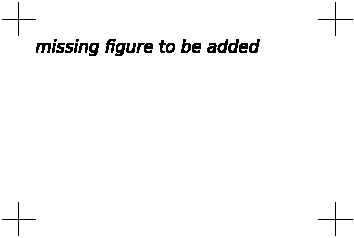
\includegraphics[height=4cm]{chapters/hoffman-1/pdf/Hoffman_fig2a.pdf}
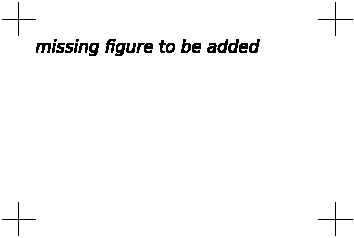
\includegraphics[height=4cm]{chapters/hoffman-1/pdf/Hoffman_fig2b.pdf}
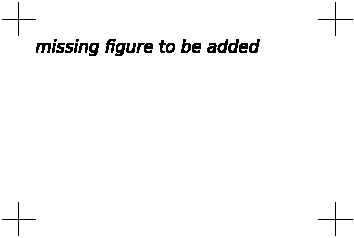
\includegraphics[height=4cm]{chapters/hoffman-1/pdf/Hoffman_fig2c.pdf}
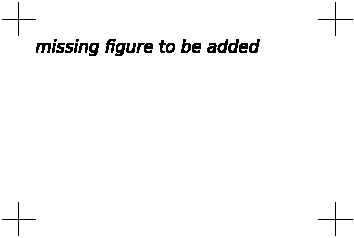
\includegraphics[height=4cm]{chapters/hoffman-1/pdf/Hoffman_fig2d.pdf}
\caption{Turbulent flow separation  \cite{JanssonHoffman2009}: velocity vectors at surface of cylinder; for $\beta = 10^{-1}$, $\beta = 10^{-2}$, $\beta = 10^{-3}$ and $\beta = 0$ (from upper left to bottom right).}
\label{fig:1}
\end{figure}

\begin{figure}
\centering
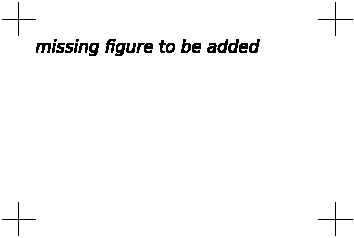
\includegraphics[height=4cm]{chapters/hoffman-1/pdf/Hoffman_fig3a.pdf}
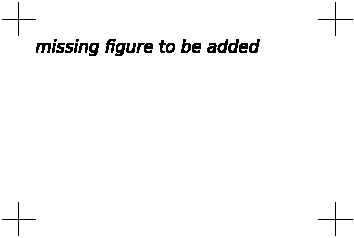
\includegraphics[height=4cm]{chapters/hoffman-1/pdf/Hoffman_fig3b.pdf}
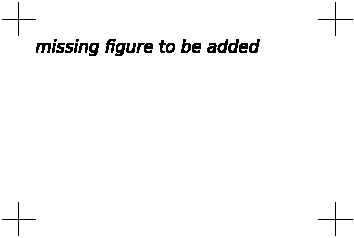
\includegraphics[height=4cm]{chapters/hoffman-1/pdf/Hoffman_fig3c.pdf}
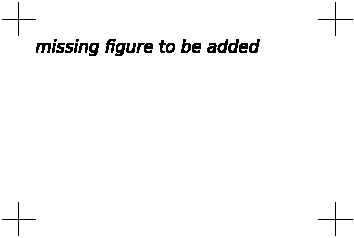
\includegraphics[height=4cm]{chapters/hoffman-1/pdf/Hoffman_fig3d.pdf}
\caption{Turbulent flow separation \cite{JanssonHoffman2009}: pressure isosurfaces; for $\beta = 10^{-1}$, $\beta = 10^{-2}$, $\beta = 10^{-3}$ and $\beta = 0$ (from upper left to bottom right).}
\label{fig:2}
\end{figure}

\begin{figure}
\centering
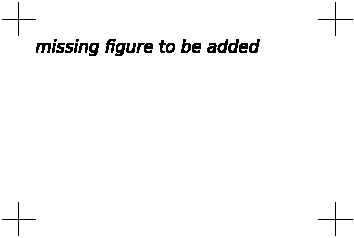
\includegraphics[height=4cm]{chapters/hoffman-1/pdf/Hoffman_fig5a.pdf}
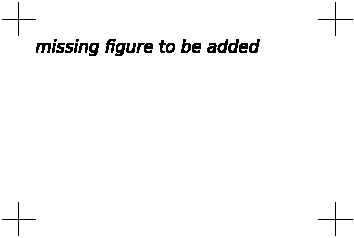
\includegraphics[height=4cm]{chapters/hoffman-1/pdf/Hoffman_fig5b.pdf}
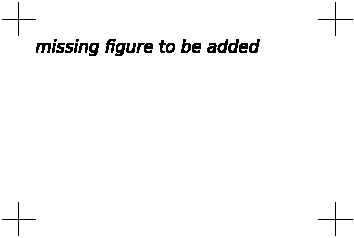
\includegraphics[height=4cm]{chapters/hoffman-1/pdf/Hoffman_fig5c.pdf}
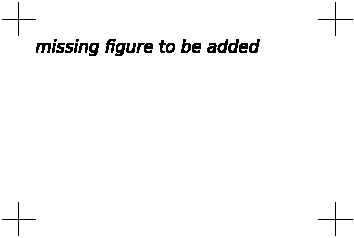
\includegraphics[height=4cm]{chapters/hoffman-1/pdf/Hoffman_fig5d.pdf}
\caption{Turbulent flow separation \cite{JanssonHoffman2009}: velocity streamlines; for $\beta = 10^{-1}$, $\beta = 10^{-2}$, $\beta = 10^{-3}$ and $\beta = 0$ (from upper left to bottom right).}
\label{fig:3}
\end{figure}

\begin{figure}[bhpt]
\centerline{
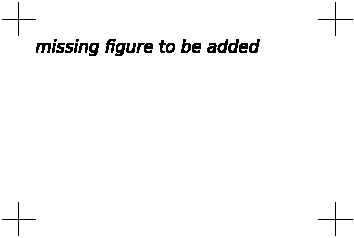
\includegraphics[height=4cm]{chapters/hoffman-1/pdf/naca_0012-vel1-aoa4-bw.pdf}
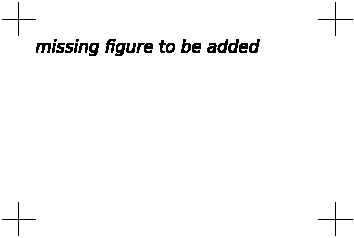
\includegraphics[height=4cm]{chapters/hoffman-1/pdf/naca_0012-vel1-aoa10-bw.pdf}
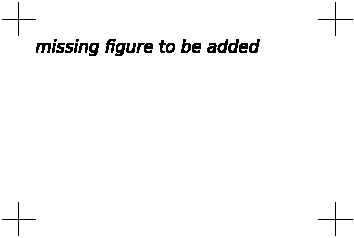
\includegraphics[height=4cm]{chapters/hoffman-1/pdf/naca_0012-vel1-aoa18-bw.pdf}
}
\centerline{
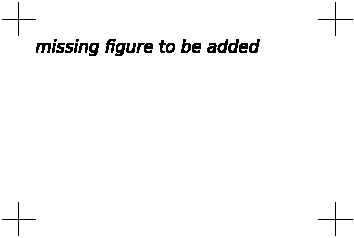
\includegraphics[height=4cm]{chapters/hoffman-1/pdf/naca_0012-aoa4-bw.pdf}
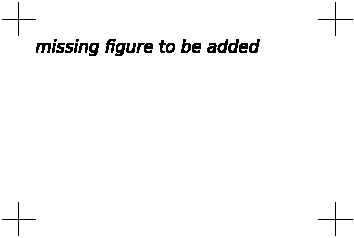
\includegraphics[height=4cm]{chapters/hoffman-1/pdf/naca_0012-aoa10-bw.pdf}
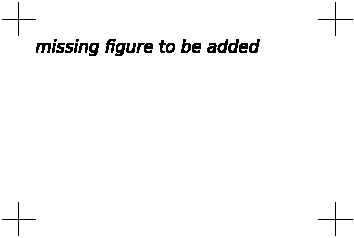
\includegraphics[height=4cm]{chapters/hoffman-1/pdf/naca_0012-aoa18-bw.pdf}
}
\centerline{
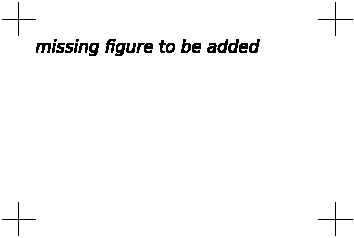
\includegraphics[height=4cm]{chapters/hoffman-1/pdf/naca_0012-vort1-xz-aoa4-bw.pdf}
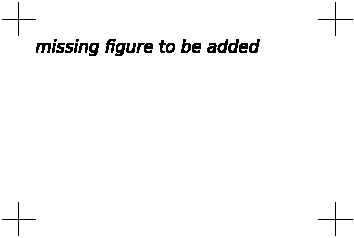
\includegraphics[height=4cm]{chapters/hoffman-1/pdf/naca_0012-vort1-xz-aoa10-bw.pdf}
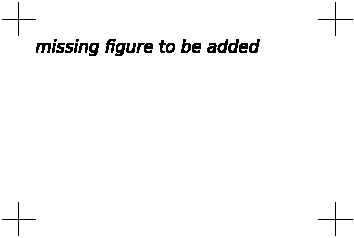
\includegraphics[height=4cm]{chapters/hoffman-1/pdf/naca_0012-vort1-xz-aoa18-bw.pdf}
}
\caption{Flow past NACA 0012 airfoil \cite{HoffmanJohnson2006}: velocity magnitude (upper), pressure (middle), and non-transversal vorticity (lower), for angles of attack 4, 10, 18$^\circ$.}
\label{fig:naca}
\end{figure}

\begin{figure}[bhpt]

\centerline{
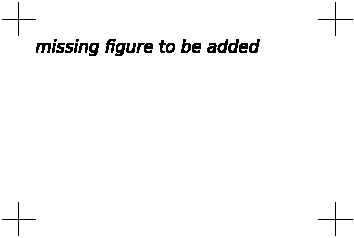
\includegraphics[width=12cm]{chapters/hoffman-1/pdf/volvo_car-bw.pdf}
}
\caption{Streamlines of turbulent flow around a car (simulations by Murtazo Nazarov, with geometry by courtesy of Volvo Cars).}
\label{fig:volvo}
\end{figure}

\subsection{Robust fluid-structure interaction}

A main challenge of fluid-structure interaction is the stability of
the fluid-structure coupling. The unified continuum model of Unicorn
provide a monolitic method which is robust, and also allows for a
flexible constitutive modeling.  As a special case of the FSI solver,
Unicorn also offers a robust solver for flow problems in deforming
domains.

There is a multitude of areas in which fluid-structure interaction
plays an important role, not the least in biomedicine that poses a
number of complex fluid-structure interaction problems.  One such
challenge is the human heart, where cardiac muscle contracts to pump
the blood through the cardiovascular system. Depending on the context
various computational models of the heart can be constructed.  To
study the fluid dynamics of the blood inside the heart, one can
reconstruct the deformation of the heart from medical imaging, to be
used as basis for a deforming domain fluid dynamics model of the blood
flow.  This is the approach underlying the simulation in
Fig.\ref{fig:heart}, where the blood flow in the left ventricle is
modeled using Unicorn. The blood is here assumed to be incompressible,
and the deforming domain is based on patient specific medical image
data. See \cite{Aechtner2009} for more details on this model.

Unicorn is designed to be able to handle large structure deformations
interacting with complex fluid flow.  In Fig.\ref{fig:flag} we present
a model problem of a flexible structure interacting with turbulent
flow in 3D, in the form of a fixed cube in high $Re$ flow with a thin
flexible flag mounted in the downstream wake.  Violent bending and
torsion motion along the long axis of the flag is observed, and we
note that the method is robust for these large structure deformations
and highly fluctuating flow.

\begin{figure}[bhpt]

\centerline{
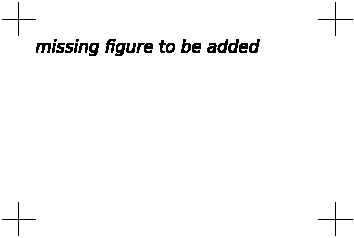
\includegraphics[width=4.5cm]{chapters/hoffman-1/pdf/pressure_animation-0020.pdf}
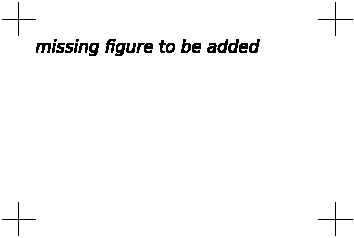
\includegraphics[width=4.5cm]{chapters/hoffman-1/pdf/pressure_animation-0064.pdf}
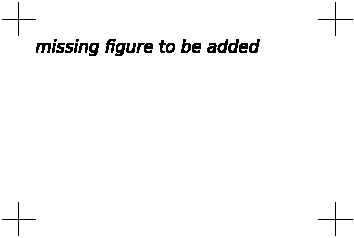
\includegraphics[width=4.5cm]{chapters/hoffman-1/pdf/pressure_animation-0135.pdf}
}

\centerline{
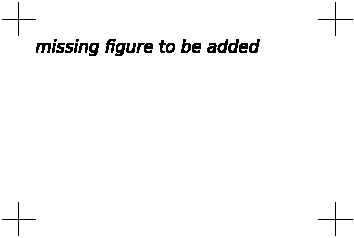
\includegraphics[width=4.5cm]{chapters/hoffman-1/pdf/velocity_animation-0020.pdf}
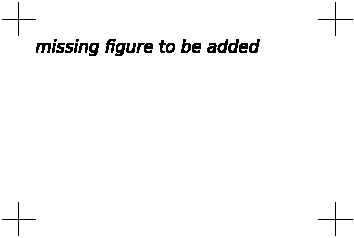
\includegraphics[width=4.5cm]{chapters/hoffman-1/pdf/velocity_animation-0064.pdf}
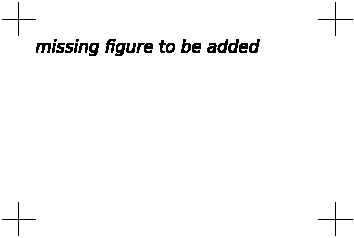
\includegraphics[width=4.5cm]{chapters/hoffman-1/pdf/velocity_animation-0135.pdf}
}
\caption{Blood flow simulation of the left ventricle of a human heart: snapshots of surface pressure (upper) and velocity (lower).
The geometrical model is constructued by Ulf Gustafsson och Per Vesterlund at Ume{\aa} Universty, and the simulations
performed by Matthias Aechtner at KTH \cite{Aechtner2009}.}
\label{fig:heart}
\end{figure}


\begin{figure}[!h]
\center{
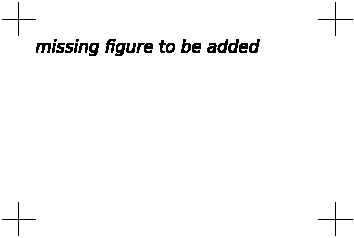
\includegraphics[width=6cm]{chapters/hoffman-1/pdf/cube000.pdf}
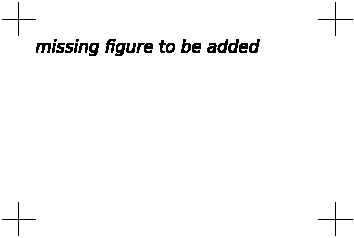
\includegraphics[width=6cm]{chapters/hoffman-1/pdf/cube115.pdf}\\
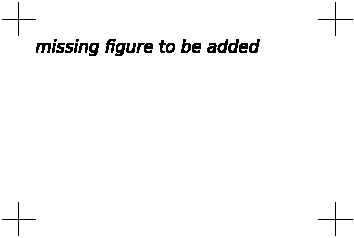
\includegraphics[width=6cm]{chapters/hoffman-1/pdf/cube125.pdf}
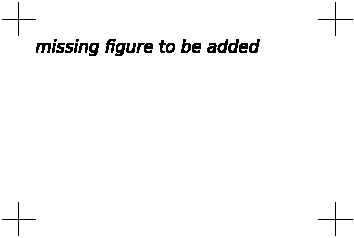
\includegraphics[width=6cm]{chapters/hoffman-1/pdf/cube168.pdf}\\
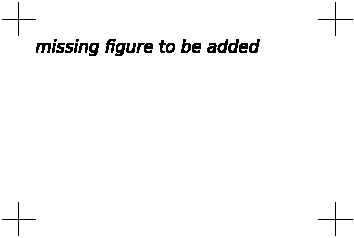
\includegraphics[width=6cm]{chapters/hoffman-1/pdf/cube187.pdf}
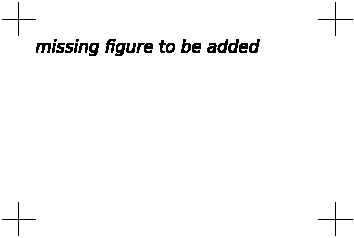
\includegraphics[width=6cm]{chapters/hoffman-1/pdf/cube405.pdf}\\
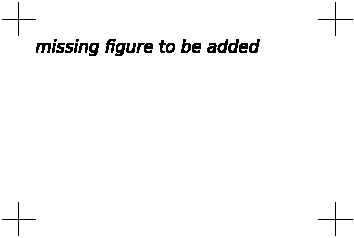
\includegraphics[width=6cm]{chapters/hoffman-1/pdf/cube550.pdf}
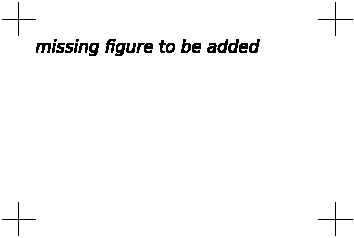
\includegraphics[width=6cm]{chapters/hoffman-1/pdf/cube649.pdf}
}
\caption{
Simulation of turbulent flow past a square cylinder with an elastic
flag attached downstream \cite{HoffmanJanssonLoggEtAl2009}: plot of cut of
the mesh, isosurface of pressure and fluid-structure phase
interface. Going from initial state top left to illustrating violent
bending and torsion motion along the long axis of the flag.  }
\label{fig:flag}
\end{figure}
